Consider a stochastic asset harvesting problem, where we have a renewable resource (e.g., a fish population) that grows according to some stochastic dynamics. The goal is to determine an optimal harvesting policy that maximizes the expected total harvest over a finite time horizon while ensuring the sustainability of the resource.

Thus, we can frame the optimal control problem as follows:
\begin{align}
    \max R = \mathbb{E}\left[ \int_{0}^{\infty} e^{-\rho t} (1 - \exp(-\alpha u_{t})) dt \right] \label{eq:harvest:objective}\\
    \text{subject to: } \quad dx_{t} = (r x_{t} - u_{t})dt + \sigma x_{t} dW_{t} \label{eq:harvest:dynamics},
\end{align}
where $x_{t}$ is the population size at time $t$, $u_{t}$ is the harvesting rate, $r$ is the intrinsic growth rate of the population, $\sigma$ is the volatility of the population growth, $\rho$ is the discount rate, and $\alpha$ controls the saturation of the harvest. The objective function represents the expected discounted total harvest over an infinite time horizon. The dynamics of the population are modeled as a stochastic differential equation (SDE) with a drift term that captures the growth and harvesting, and a diffusion term that captures the stochastic fluctuations in the population size.

For this example, we define the following parameters:
\begin{align*}
    r &= 0.5 \quad \text{(intrinsic growth rate)}\\
    \sigma &= 0.1 \quad \text{(volatility)}\\
    \rho &= 0.05 \quad \text{(discount rate)}\\
    \alpha &= 0.5 \quad \text{(saturation parameter)}
\end{align*}

\subsection{Baseline/Ground Truth Solution}
We know that the optimal harvesting policy can be derived from the Hamilton-Jacobi-Bellman (HJB) equation associated with this problem. The HJB equation for this problem is given by:
\begin{align}
    \rho V(x) &= \max_{u} \left\{ (1 - \exp(-\alpha u)) + V'(x)(r x - u) \right.\nonumber\\
    &\qquad \left. + \frac{1}{2} \sigma^2 x^2 V''(x) \right\}\label{eqn:harvest:hjb}
\end{align}
where $V(x)$ is the value function representing the maximum expected discounted harvest starting from population size $x$. The optimal harvesting policy can be obtained by solving the HJB equation numerically using a PDE solver or classical value iteration methods. This solution will serve as our baseline or ground truth for evaluating the performance of the value function learning methods discussed in this survey.

\subsection{Results}
For each method, we compute an RMSE between the learned value function and the ground truth solution obtained from solving the HJB equation. The results are summarized in Table~\ref{tab:harvest_results}. We can see that the Deep BSDE method achieves the lowest RMSE, indicating that it learns a value function that is closest to the ground truth. The ADP (Actor-Critic) method also performs reasonably well, while the PINN/DGM method has a higher RMSE. The Neural Value Iteration method diverges significantly in this case, resulting in a very high RMSE.

\begin{table}[h]
\centering
    \begin{tabular}{|c|c|}
        \hline
        \textbf{Method} & \textbf{RMSE} \\
        \hline
        PINN / DGM & 3.297 \\
        Deep BSDE & 0.933 \\
        ADP (Actor-Critic) & 2.084 \\
        Neural Value Iteration & 6247.684 \\
        \hline
    \end{tabular}
    \caption{RMSE between learned value functions and ground truth solution for the stochastic asset harvesting problem.}
    \label{tab:harvest_results}
\end{table}

We visualize the learned value functions and the corresponding optimal harvesting policies derived from each method in Fig.~\ref{fig:asset_harvesting_results}. The value function plots (on the top) show how well each method approximates the true value function across different population sizes. The policy plots (on the bottom) show the optimal harvesting rate as a function of the population size, which should ideally reflect the trade-off between harvesting and sustainability. \textcolor{red}{The top plot is currently biased by the results of the NVI, which has completely diverged.}

The bottom plot shows the corresponding optimal harvesting policies derived from the learned value functions. We can see that all the methods do not learn the policy well.


\begin{figure}
    \centering
    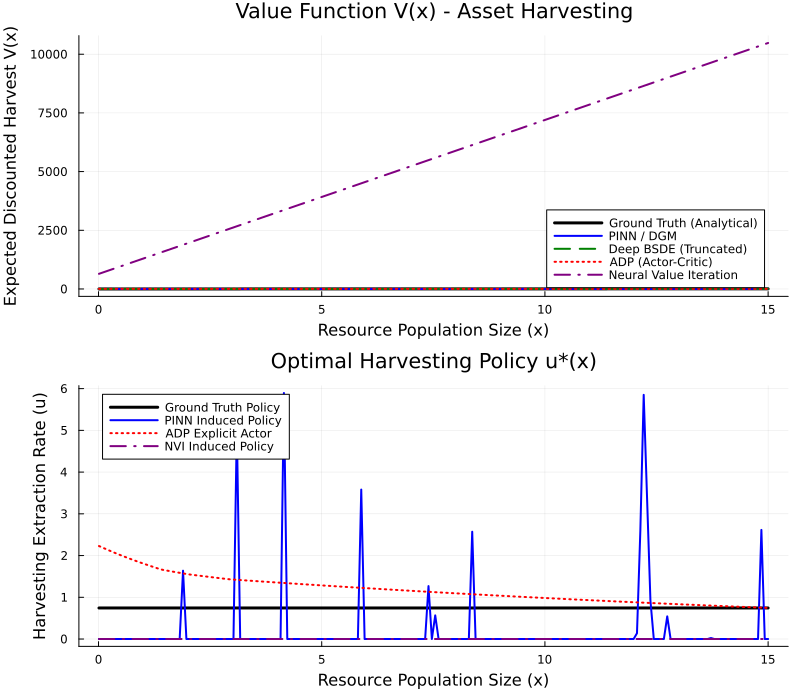
\includegraphics[width=\columnwidth]{code/figures/value_function_benchmark_comparison.png}
    \caption{Learned value function (top) and optimal harvestin strategy (bottom).}
    \label{fig:asset_harvesting_results}
\end{figure}

\textcolor{red}{TODO: Add more discussion on the results, especially the policy plots. Also, we should investigate why the NVI method diverged so significantly in this case.}